\section{Preliminary Applications Results}
    \label{sec:perf}
    \subsection{Platform Description}
    \label{subsec:ec2}
    Our tests use the new HPC-oriented Amazon EC2 Cluster Compute Instances
    (CCIs) available since July 2010. Each CCI has 2 quad-core Intel Xeon
    X5570 "Nehalem" processors, with 23GB of memory. Each instance is
    allocated to users in a dedicated manner, unlike those in most other EC2
    instance classes \cite{amazon:hpc}. The CCIs are interconnected with 10
    Gigabit Ethernet. Due to the unstable availability of EBS storage that we
    recently encountered, all our experiments in this section use the
    ephemeral disks. 

    Regarding software settings, we use the Cluster Instances Amazon Linux AMI
    $2011.02.1$ associated with CCIs, the Intel compiler $11.1.072$ and Intel
    MPI $4.0.1$. The default compiler optimization level is \emph{$-O3$}.

    \subsection{Selected HPC Applications}
    Our experiments evaluated two parallel applications. BTIO is the
    I/O-enabled version of the BT benchmark in NPB suite \cite{wong:btio}.
    The program solves Navier-Stokes equations in three spatial dimensions,
    which are discretized, unsteady and compressible. Each of the processor
    will be in charge of multiple Cartesian subsets of entire data set. The
    I/O strategy employs collective buffering and writing via MPI-IO
    interface, to avoid heavy fragmentation caused by writing per-process
    output files. The default I/O frequency is used, appending to the shared
    output file every 5 computation time steps, resulting in an output file
    sized around 6.4GB.  The BT problem size was class C for all the tests,
    built with \texttt{FULL} subtype. POP is an ocean circulation model which
    solves the three-dimension primitive equations for fluid motions on the
    sphere \cite{website:pop} and exhibits a read-once-write-many I/O pattern.
    It reads a setup file at the initialization phase and performs write
    operation in native Fortran I/O interface at each period time step. We
    used the POP grid dimensions of 320x384x20 and the total output size is
    about 6GB, aggregated and written by process 0.

    \subsection{BTIO Results}
    In this section, we present the performance and total computation cost of
    running BTIO on EC2 CCIs, using NFS (\textit{async} mode) and PVFS
    respectively. For each storage option, we also present the performance
    difference between two I/O server placement modes: I/O servers occupy
    separate compute instances under the \textit{dedicated} mode, and
    co-reside instances with compute processes under the \textit{part-time}
    mode.
    \begin{figure}[htpb]
        \centering
        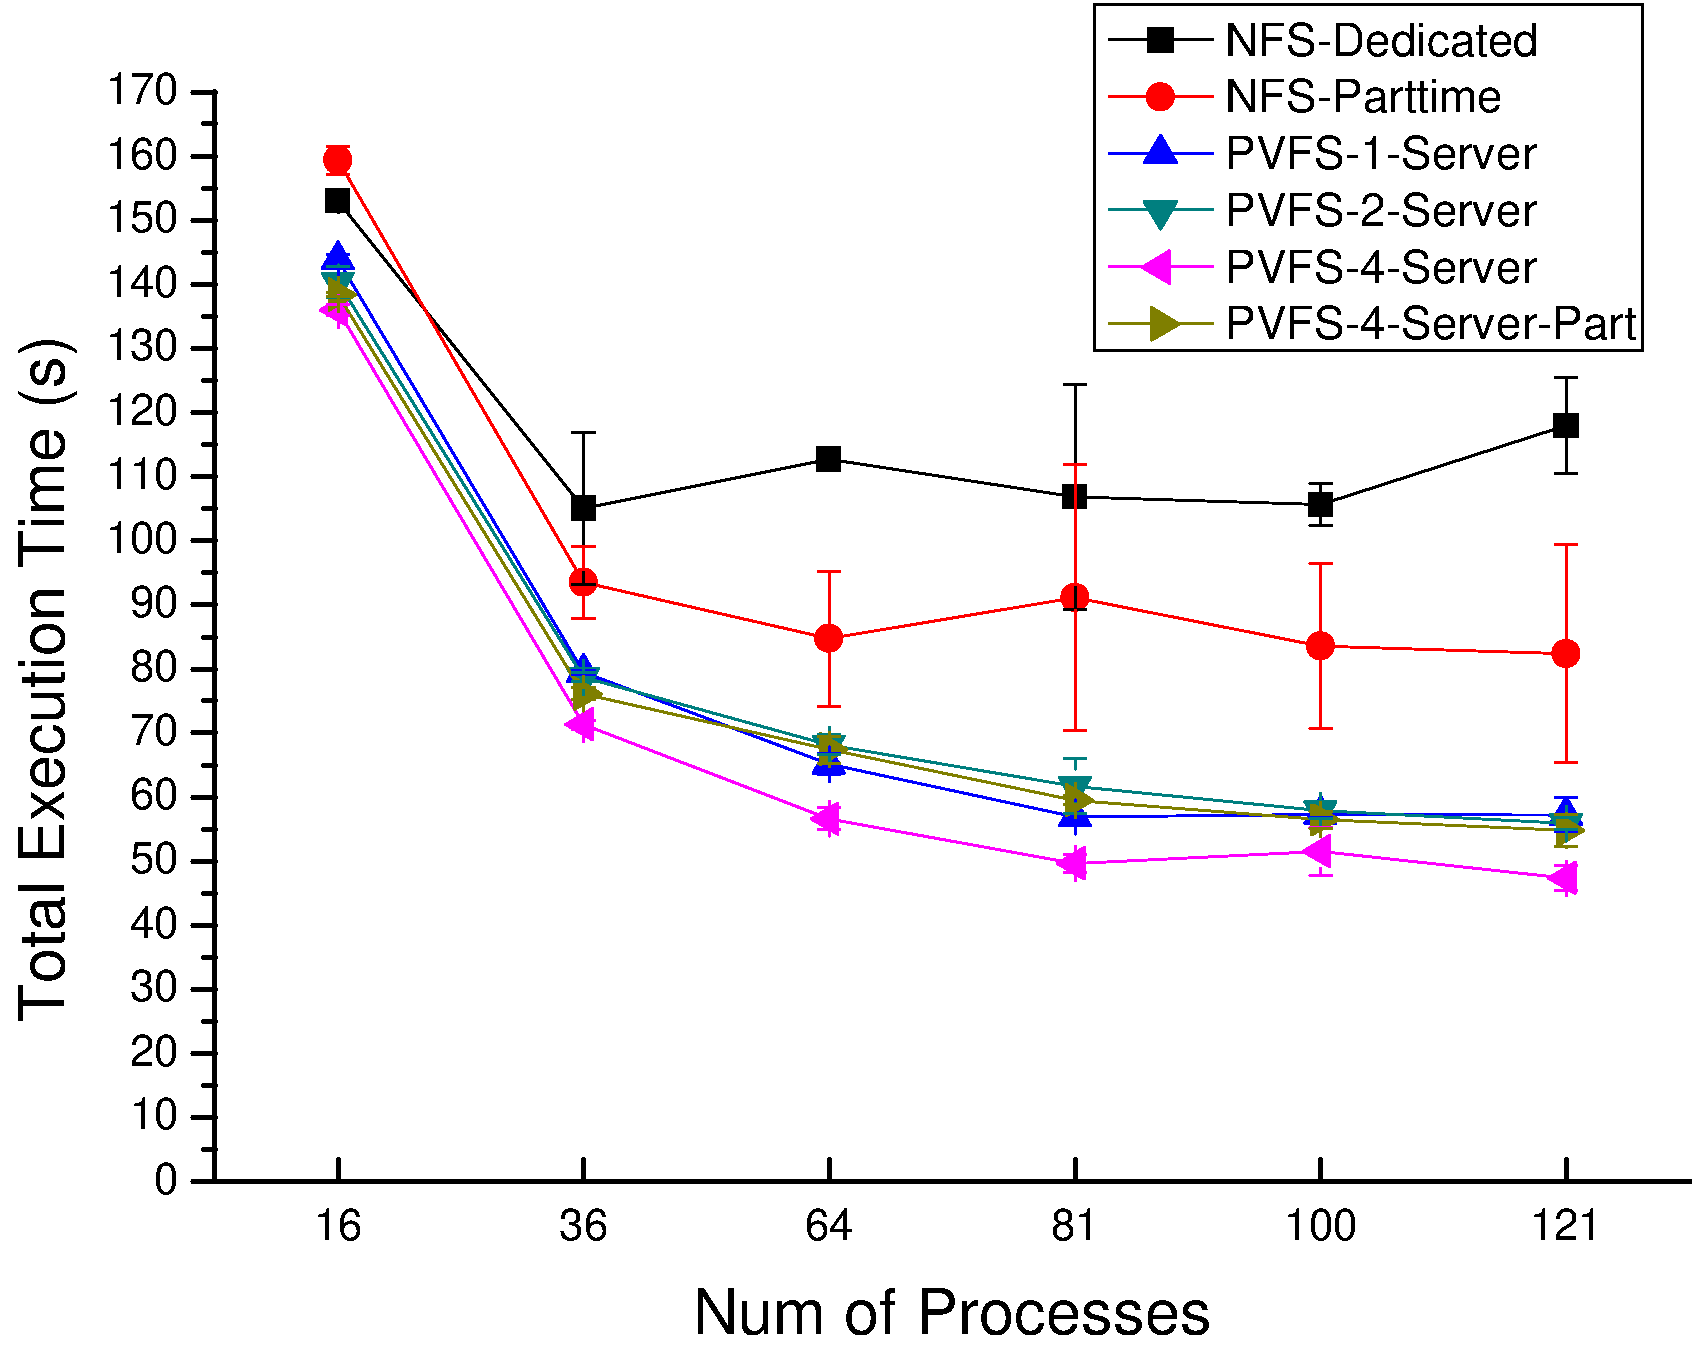
\includegraphics[width=0.8\linewidth]{../figures/T-time}
        \caption{BTIO total execution time}
        \label{fig:bt-time}
    \end{figure}

    Figure~\ref{fig:bt-time} shows the total execution time of BTIO under
    different file system configurations. There are up to 4 I/O servers, each
    mounting two ephemeral disks with software RAID0. For PVFS,
    one of the I/O servers acts as the meta-data server. From the results, we
    can see that for BTIO, PVFS beats NFS in all test cases. For example,
    there is an up to 60\% performance improvement from using NFS (with one
    dedicated server) to using PVFS (with 4 dedicated servers). The
    performance gain is more likely due to the collective MPI-IO optimizations
    contained in the PVFS design, as even with just one I/O servers, PVFS
    significantly outperforms NFS. Also, the NFS performance appears to have a
    much higher variance compared to that of PVFS. Interestingly, NFS performs
    better when the I/O server runs in the part-time mode, which can be partly
    attributed to the enhanced data locality and reduced network contention.
    However, we doubt that this factor alone causes the large performance
    difference observed and are carrying out more detailed investigation.

    Judging by the I/O bandwidth measured from BTIO, PVFS performance scales
    well with increased number of I/O servers (results not plotted due
    to space limit). However, the scalability does not reflect well in
    Figure~\ref{fig:bt-time}, the overall performance chart. This is due to
    the total portion of execution time devoted to I/O. For this strong-scaling
    experiment we expect to see that I/O gains more weight in the execution
    time, but the computation component of BT does not scale well on Amazon
    EC2, due to the unsatisfactory interconnection. Therefore as the number of
    processes increases, the total percentage of time spent on I/O is
    maintained at around 10\%.
    \begin{figure}[htpb]
        \centering
        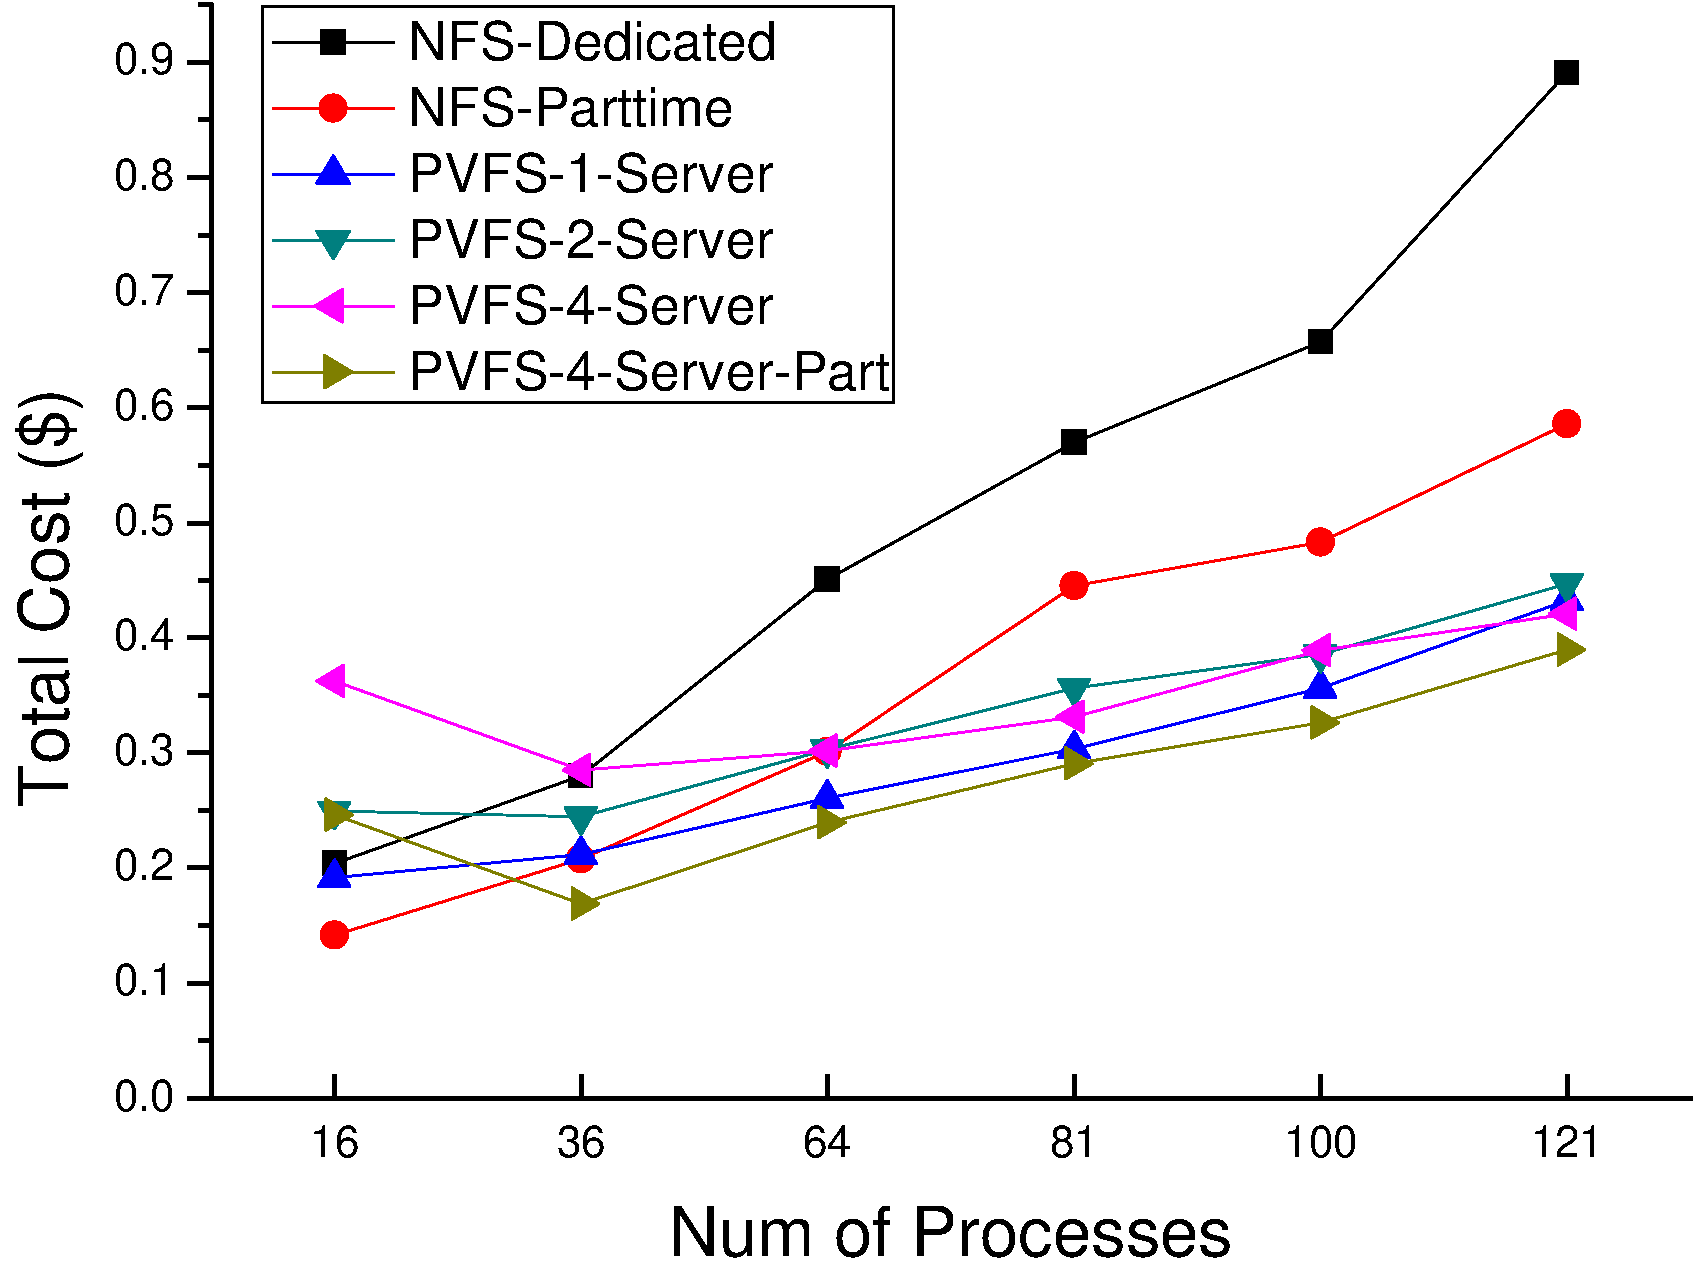
\includegraphics[width=0.8\linewidth]{../figures/T-cost}
        \caption{The total cost of BTIO executions}
        \label{fig:bt-cost}
    \end{figure}

    A related issue is the total cost of execution, when we factor in the
    total number of instances needed. Figure~\ref{fig:bt-cost} shows the cost
    comparison derived from the BTIO results, using the Amazon
    charging rate of \$1.6 per instance per hour. Here we can see the appeal
    of using part-time I/O servers. In addition, at a small execution scale,
    NFS with one part-time server actually appears to be the most
    cost-effective option.

    \subsection{POP Results}
    We run POP with similar I/O configurations (Figure~\ref{fig:pop}). 
    Unlike with BTIO, here NFS (\textit{async} mode at server side)
    outperforms PVFS across all configurations. There are several possible
    reasons. First, POP has process 0 carry out all I/O tasks, making the
    parallel I/O support that PVFS was designed for less useful and the
    network communication more bottleneck-prone in I/O.  Second, POP does I/O
    via POSIX interfaces, which is not optimized in PVFS. Due to its heavy
    communication with small messages, POP does not scale on EC2, as can be
    seen from Figure~\ref{fig:pop}. However, its I/O behavior is still
    representative in parallel applications.
    \begin{figure}[htpb]
        \centering
        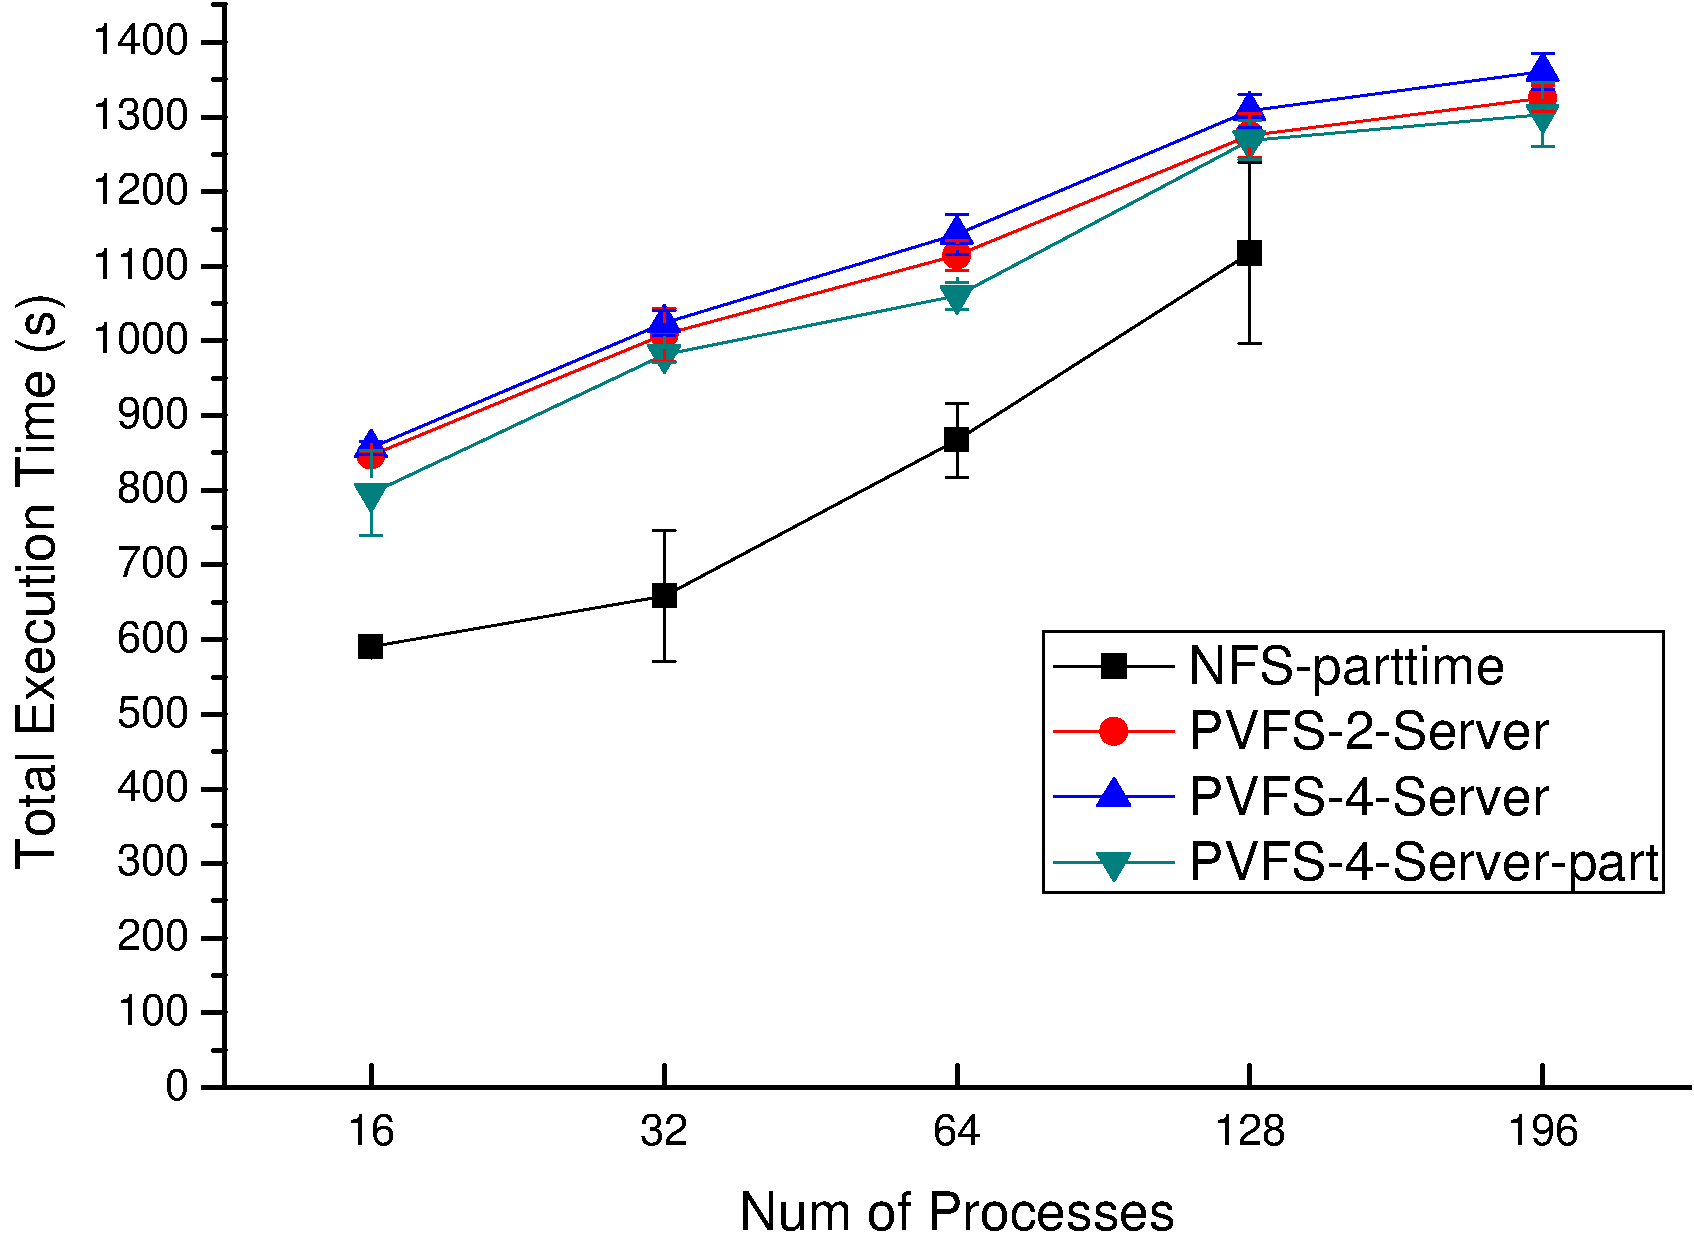
\includegraphics[width=0.8\linewidth]{../figures/pop}
        \caption{POP total execution time}
        \label{fig:pop}
    \end{figure}
